\documentclass[border=2mm]{standalone}
\usepackage{pgfplots}
\usepackage[scaled]{helvet}
\usepackage[T1]{fontenc}
\renewcommand\familydefault{\sfdefault}
\usepackage[eulergreek]{sansmath}
\pgfplotsset{
tick label style = {font=\sansmath\sffamily}}

\pgfkeys{/pgf/number format/fixed}
\pgfplotsset{compat=newest}
\begin{document}

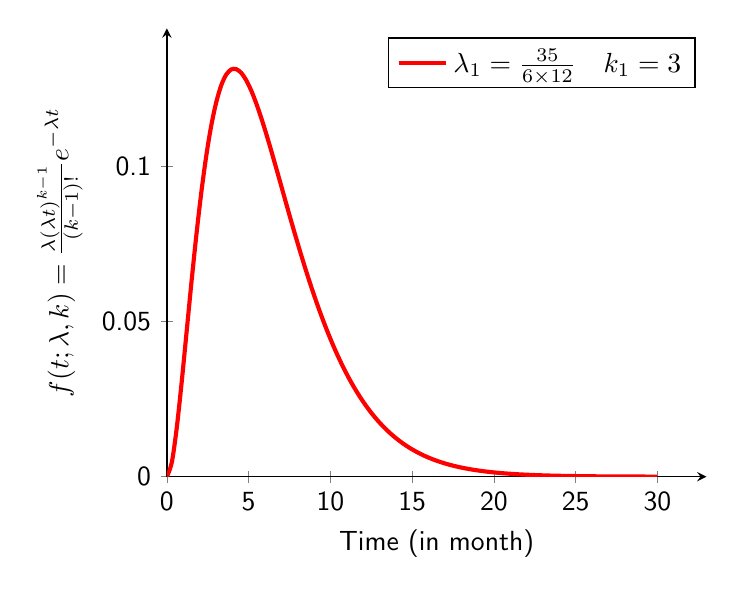
\begin{tikzpicture}
\begin{axis}[
    scaled ticks=false,
    axis lines=left,
    enlargelimits=upper,
    line width=0.5,
    legend entries={$\lambda_1=\frac{35}{6\times 12}\quad k_1=3$},
    xlabel = Time (in month),
    ylabel = {$f(t;\lambda,k)=\frac{\lambda(\lambda t)^{k-1}}{(k-1)!}e^{-\lambda t}$}
]
\addplot + [smooth, mark=none, domain=0:30, samples=100, color=red, line width=1.5] { ((35/(6*12)*(35/(6*12)*x)^(3-1))*exp(-35/(6*12)*x)/factorial(3-1)};
\end{axis}
\end{tikzpicture}
\end{document}